\chapter{A framework for diversity analysis of whole shotgun metagenomic reads data}



\section{Introduction}



Here we propose a novel concept, ``informative genomic segment'' or IGS,
and use IGS as a replacement of OTUs as the basic unit for 
diversity analysis of whole shotgun metagenome data sets. IGSs represent the 
unique information in a metagenomics data set and the abundance of IGSs in 
different samples can be retrieved by analyzing read coverage with an efficient 
k-mer counting method (discussed in the previous two chapters).
The samples-by-IGS abundance data matrix is a promising
replacement of samples-by-OTU data matrix used in 16S rRNA based analysis and 
many existing statistical methods can be applied to work on the samples-by-IGS 
data matrix to investigate diversity. We applied this method to
several simulated data sets and several real metagenomic data sets, including
human microbiome, sea water and soil data. The results of beta diversity analysis
showed that the samples were clustered with comparable or better accuracy than 
existing alignment-based method. The results of alpha diversity analysis 
showed this was a promising new approach to estimate metagenome sizes.
Since this method is totally binning-free, 
assembly-free, annotation-free, and reference-free, it is promising 
for dealing with highly diverse environmental samples, where we are facing
many unknowns.



\section{The concept of IGS(informational genomic segment)}

In classic ecology dealing with macroorganisms, diversity measurement is based 
on the concept of species. For 16S rRNA amplicon metagenomics data set, it is 
based on the concept of OTUs. While the concept of OTUs can be used to analyze
large shotgun metagenomics data set, normally assembly, binning and annotation
are required before doing diversity analysis. However for many metagenomics 
projects these are difficult
tasks, lacking necessary reference genome or requiring expensive
computation. So we are interested in finding an approach to bypass difficult
tasks like assembly, binning, annotation and use the raw reads to make the 
diversity analysis of large shotgun whole genome metagenomic data possible. 
% @CTB citations for this paragraph?

We began such efforts by proposing that
 the concept of k-mer (a DNA segment with the length of k) could be used as the 
 basic unit to measure
the diversity. K-mers can be considered as the atom of information in DNA 
sequences. One of the composition-based approaches to binning is to use the 
k-mers as the source of signatures\cite{Alneberg2014, Imelfort2014}. Suppose the sizes of microbial genomes are similar and
 the difference between genomic content of microbial genomes is similar, the 
number of distinct k-mers in the sequence data set correlates to the number of 
species in a sample. However, because of sequencing error, which is unavoidable
 due to the limit of sequencing technology, this k-mer based analysis does not 
work well on unassembled data. One sequencing error on a read will generate up to  k erroneous 
k-mers. In metagenomics data sets, especially with high coverage, most of the 
distinct observed k-mers are from sequencing errors.
%add citation about k-mer based diversity analysis ,entropy...
% add some results /figures

Next we shifted the focus from k-mers onto a higher level - reads. 
In previous chapter, we have discussed a novel approach to use median k-mer 
count in a read to estimate
sequencing depth without a reference assembly, based on which the framework for
streaming analysis of short DNA sequencing reads was developed.
It also offers a novel way to distill information from reads by reducing the
 bad effect of sequencing errors so that we can use those informative reads to 
measure the microbial diversity. We term those informative reads as 
IGSs (informative genomic segments), which can be considered segments of DNA 
on a microbial genome. Those IGSs should be different enough to represent the 
abstract information a genome contains. Suppose microbial genomes contain 
similar number of those IGSs, as they contain similar number of distinct 
k-mers; then the number of IGSs will correlate with the species richness in a 
sample, and the abundance distribution of IGSs will be related to species 
evenness in a sample. Furthermore, we can get the abundance of the IGSs across
different samples. Many classic diversity estimation methods based on OTUs 
 described in the literature review chapter can be applied to estimate 
 the diversity of IGSs 
and the diversity of actual species subsequently.


% need expanding
For alpha diversity, we can generate a list of IGSs and the respective 
abundance in a sample. Then existing estimators like Chao's can be applied to 
estimate the total number of IGSs in the sample. Rarefaction curves based on the
number of IGSs can also be generated. 

% need expand the discussion from IGS in one sample to IGS in different samples.
For beta diversity, we can generate a samples-by-IGS data matrix from the
abundance of IGSs across samples, as a replacement of samples-by-OTU data 
matrix in OTU-based analysis and samples-by-species data matrix in traditional 
ecology. From that samples-by-IGS data matrix, we can use existing methods to 
calculate similarity/dissimilarity/distance between samples and do further 
analysis like clustering and ordination. 


\subsection{IGS(informative genomic segment) can represent the novel 
information of a genome}

Median k-mer abundance can represent sequencing depth of a read, as discussed
in last chapter (published as \cite{Brown2012}).
 For a sequencing reads data set with multiple species, the sequencing depth of
 a read is related to the abundance of species where the read originates from. 

% figure 1a should be marked 
The upper plot in Figure \ref{fig:reads_to_IGS} shows the abundance distribution of reads 
from 4 simulated sequencing data sets with different sequencing depths - 3 
sequencing data sets generated with different sequencing coverage(1x, 10x, 40x)
 from 3 simulated random genomes respectively and 1 combined data set with all 
the aforementioned data sets. No error is introduced in these simulated 
data sets. Obviously the reads from the three data sets can be separated by 
estimated sequencing depth. The combined data set can be considered as a 
sequencing data set with three species with different abundance.

Each point on the curve shows that there are $Y$ reads with a sequencing depth of
 $X$. In other word, for each of those $Y$ reads, there are $X-1$ other reads that 
cover the same DNA segment in a genome that single read originates. So we can 
estimate that there are $Y/X$ distinct DNA segments with reads coverage as $X$. 
We term these distinct DNA segments in species genome as 
IGSs (informative genomic segments). We can transform the upper plot in 
Figure \ref{fig:reads_to_IGS} to show the number of IGSs and their respective 
reads coverage, as 
shown in lower plot. We sum up the numbers of IGSs with 
different reads coverage for each data set and get the result as shown in 
Table \ref{table:IGSs}. The sum numbers of IGSs here essentially are the areas below each curve 
in the figure.

Even though the datasets have different sequencing depth like 10X and 40X, 
they have similar numbers of IGSs. Dataset with 1X sequencing depth has fewer 
IGSs because the depth is not enough to cover all the content of the 
genome(63.2\%). The IGSs can be seen as the
genomic segments on a genome with the length of reads.(Figure \ref{fig:IGS}  
Assume the composition of species 
genome is totally random, which is the case in the simulated data sets, the 
number of IGSs (N) in a species genome is related to the size of genome(G), 
read length(L) and k size(k), which can be denoted as

\[N =\frac{G}{L}  \]
which is the number of reads that can have a 1X coverage of the genome.
For the simulated genome with size of 1M bps, read length as 80bps, expected 
number of IGSs is 

\[1000000/80 = 12500 \], 

which is close to the observed value. See Table \ref{table:IGSs}


\begin{figure}[!ht]
\centerline{\includegraphics[width=4in]{./figures/from_reads_to_IGS.png}}
\caption{\bf Transforming reads into IGSs.}
\label{fig:reads_to_IGS}
\end{figure}

\begin{table}[!ht]
\caption{
\bf{Total number of IGSs in different simulated reads data sets.}
}
\begin{tabular}{ |c | c |c| c|c| }
Data set & total number of IGSs \\
\hline 
1X depth                   & 6419  \\
10X depth                  & 12022  \\
40X depth                  & 12371 \\
1X,10X,40X combined        & 30748 \\
\end{tabular}
\begin{flushleft}
\end{flushleft}
\label{table:IGSs}
\end{table}


\begin{figure}[!ht]
\centerline{\includegraphics[width=4in]{./figures/IGSs_figure.pdf}}
\caption{\bf IGS(informative genomic segment) can represent the novel information of a genome.}
\label{fig:IGS}
\end{figure}





\subsection{Using IGS to analyze alpha diversity}

Basically the abundance distribution of IGSs with different coverage in a 
sample data set can be acquired using the method shown above.

Suppose from a reads data set, the coverage distribution of reads is as 
shown in this table: %Table \ref{table:read_coverage}.
\\
%\begin{table}[!ht]
\begin{tabular}{|c|c|c|c|c|}
coverage & number of reads \\
\hline 
%&\\
3                   & 69  \\
4                  & 96  \\
5                  & 125 \\
6                   & 150 \\
...        & ... \\
\end{tabular}
\begin{flushleft}
\end{flushleft}
%\caption{\bf Reads coverage distribution.}
%\label{table:read_coverage}
%\end{table}

There are 69 reads with coverage as 3, 96 reads with coverage as 4, 
and so on. We transform this coverage distribution
of reads into abundance distribution of IGSs, as shown in this table: %Table \ref{table:igs_coverage}.
\\
%\begin{table}[!ht]
\begin{tabular}{ |c | c |c| c|c| }
abundance & number of IGS \\
\hline 
%&\\
3                   & 23  \\
4                  & 24  \\
5                  & 25 \\
6        & 25 \\
...        & ... \\
\end{tabular}
\begin{flushleft}
\end{flushleft}
%\caption{\bf IGS abundance distribution.}
%\label{table:igs_coverage}
%\end{table}

For example, there are 23 IGSs with abundance 3. This is calculated by dividing  
total number of reads with coverage as 3, which is 69, by the coverage 3.
Similarly there are 24 IGSs with abundance 4. 
If we draw an analogy between IGSs and OTUs, this is like saying there are 23 
different OTUs with 3 reads mapped to each OTU, and 24 different OTUs with 4 reads mapped to each OTU, and so on.

Next all the different IGSs and the corresponding abundances can be listed,
as shown here: %able \ref{table:igs_abundance}. 
\\
%\begin{table}[!ht]
\begin{tabular}{ |c | c |c| c|c| }
IGS ID & abundance \\
\hline 
%&\\
1                   & 3  \\
1                 & 3  \\
1                  & 3 \\
...        & ... \\
23        & 3 \\
24        & 4 \\
25        & 4 \\
...        & ... \\
47        & 4 \\
48        & 5 \\
...        & ... \\
\end{tabular}
\begin{flushleft}
\end{flushleft}
%\caption{\bf Listing IGSs with the corresponding abundances.}
%\label{table:igs_abundance}
%\end{table}

This list is the counterpart of an 
OTU table in OTU based diversity analysis.
With such table at hand, existing statistical methods and software 
packages can be directly used to investigate the alpha diversity.  

\subsection{Using IGS to analyze beta diversity}

As with alpha diversity analysis, the OTU table is also a foundation for beta 
diversity analysis. As long as we get a reliable OTU table, there are existing 
pipelines to perform the beta diversity analysis. 

A typical OTU table across different samples is like this, which is also 
called a samples-by-OTU data matrix:%(Table \ref{table:OTU_table})
\\
%\begin{table}[!ht]
\begin{tabular}{ |c | c |c| c|c| }
    OTU ID & Sample A & Sample B & Sample C \\
\hline 
%&&\\
OTU1 & 3 & 4 & 2  \\
OTU2 & 2 & 5 & 0 \\
OUT3 & 3 & 1 & 4 \\
...  & ... & ... & ... \\
\end{tabular}
\begin{flushleft}
\end{flushleft}
%\caption{\bf Samples-by-OTU matrix.}
%\label{table:OTU_table}
%\end{table}

Like a OTU table, we hope to have the IGS table for the IGSs: %(Table \ref{table:IGS_table})
\\
%\begin{table}[h]
\begin{tabular}{ |c | c |c| c|c| }
    IGS ID & Sample A & Sample B & Sample C \\
\hline 
%&&&\\
IGS1 & 2 & 3 & 2  \\
IGS2 & 2 & 4 & 0 \\
IGS3 & 3 & 3 & 4 \\
...  & ... & ... & ... \\
\end{tabular}
%\caption{\bf Samples-by-IGS matrix.}
%\label{table:IGS_table}
%\end{table}
\\



\begin{figure}[!ht]
 \centerline{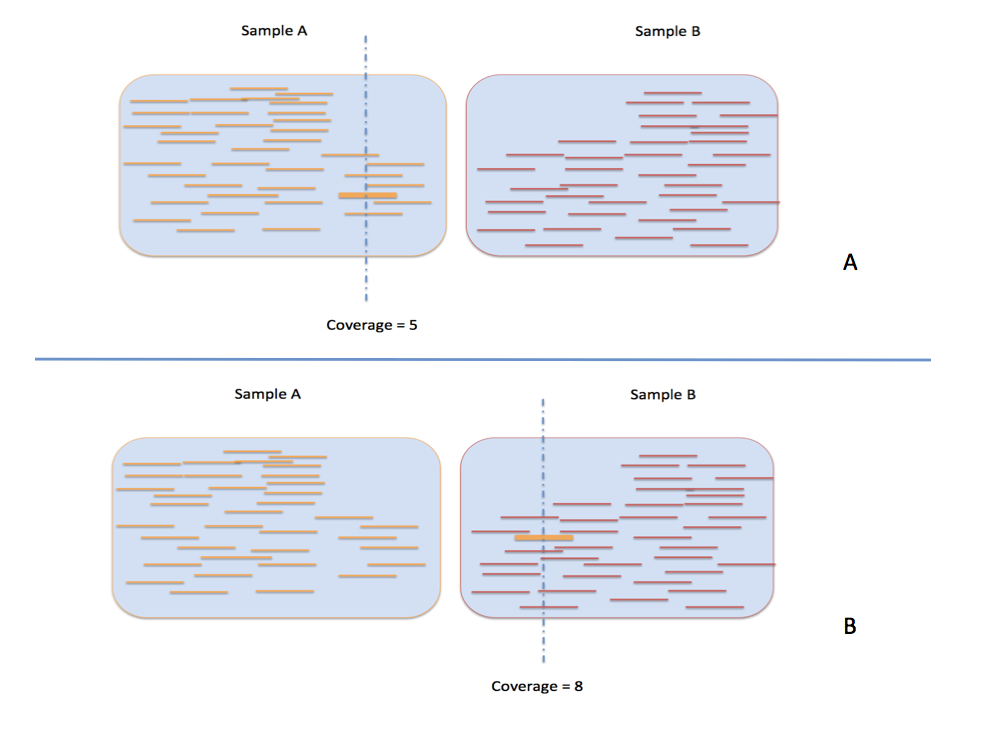
\includegraphics[width=7in]{./figures/read_coverage_samples.png}}
\caption{\bf Get the coverage of a read in samples. A read in sample A has the coverage of 5 in sample A, has
the coverage of 8 in sample B.}
\label{fig:read_coverage_samples}
\end{figure}



    
So now the problem is how we can generate a samples-by-IGS matrix as 
the counterpart of samples-by-OTU matrix so many of the existing 
tools/methods used for OTU-based diversity analysis can be borrowed for this kind 
of IGS-based analysis, just as what is shown above for alpha diversity analysis.

Firstly, using the same approach to get the coverage of a read in the sample data set where it is from 
(Figure \ref{fig:read_coverage_samples}-A), we can get the coverage of a read from sample A dataset in 
 sample B dataset (Figure \ref{fig:read_coverage_samples}-B). We still use the median k-mer count to represent 
the coverage of a read.  

\begin{figure}[!ht]
 \centerline{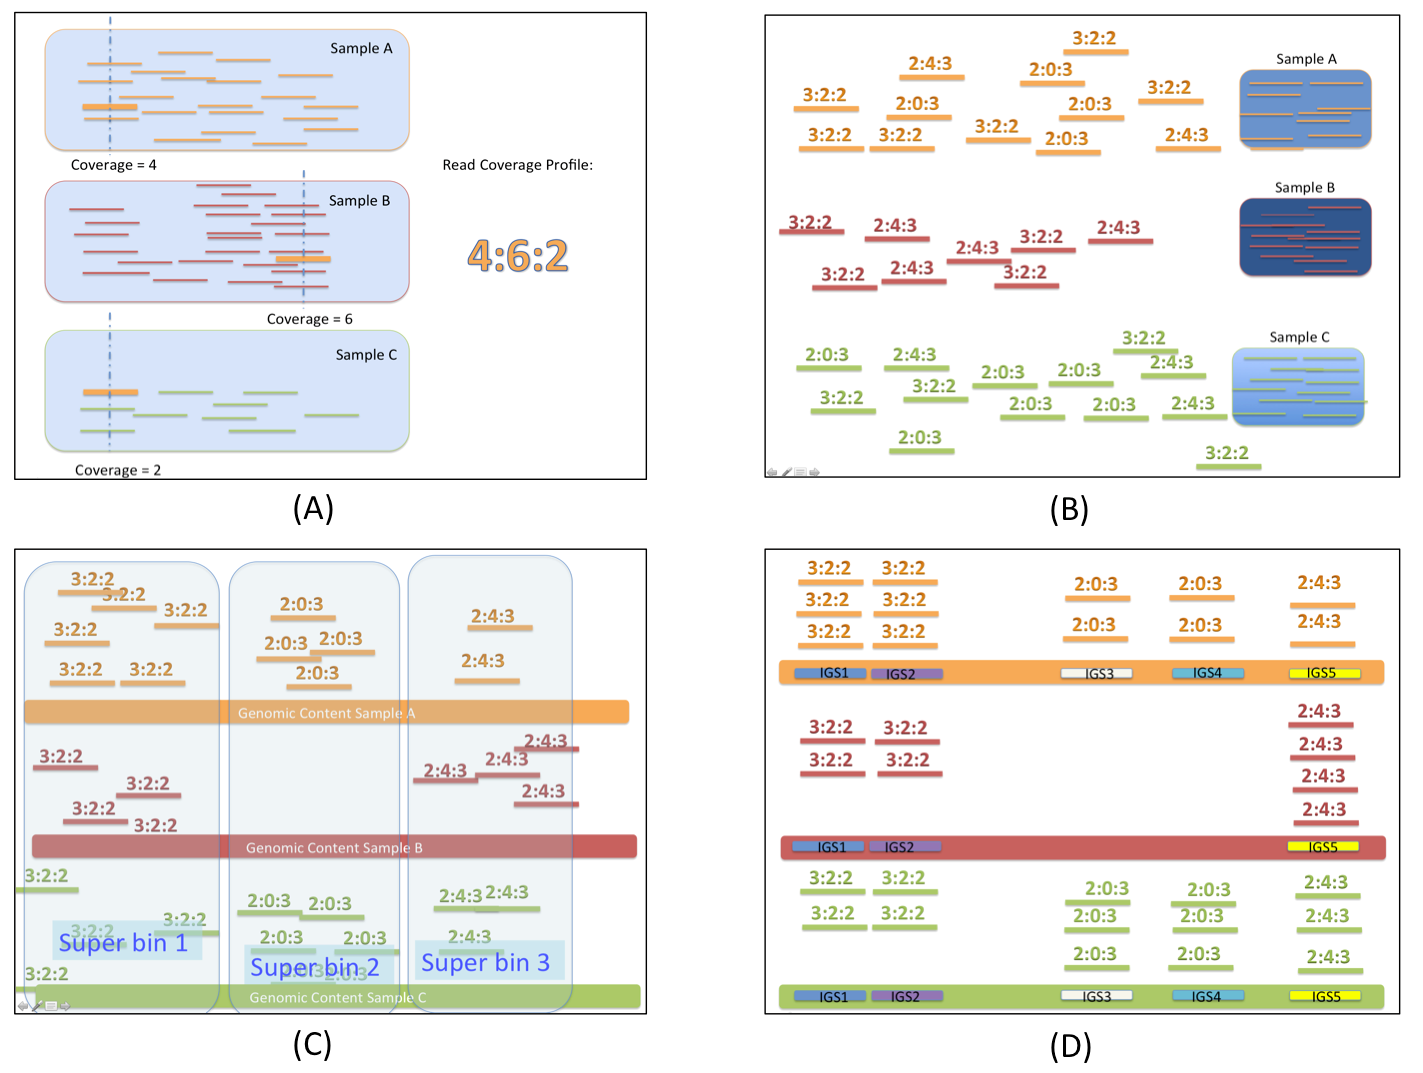
\includegraphics[width=7in]{./figures/coverage_profile.png}}
 \caption{\bf From read coverage profile to IGS. (A): Get the coverage profile of one read. (B): Get the coverage
 profiles of all the reads in 3 samples. (C): Group the reads with same coverage profiles into ``super bin''. 
 (D): Calculate the number of IGSs in each ``super bin''.}
\label{fig:coverage_profile}
\end{figure}

For a data set with several samples to analyze, firstly we can get the coverage of a read across different samples and get a read coverage
profile like ``4:6:2'', as shown in Figure \ref{fig:coverage_profile}(A). 
For all the reads in the samples we can get such read coverage profiles, as 
shown in Figure \ref{fig:coverage_profile}(B). 
We have already known that "contigs with similar coverage profiles are likely
to have originated from the same microbial population"\cite{Imelfort2014}.
Several new binning methods based on coverage profiles have been developed
based on such assumption\cite{Albertsen2013,Karlsson2013,Alneberg2014,Nielsen2014,Imelfort2014}.
Thus, here we can assume that reads with similar coverage profiles are 
likely to have originated from the same genomic region. Actually it is safer to 
say reads with different coverage profiles are not likely to have originated from
the same genomic region. The next step is to group those reads with same
coverage profiles together into ``super bin'' in different samples, as shown 
in Figure \ref{fig:coverage_profile}(C). The reads in each ``super bin'' may 
not be from the same species, but they should be from the species that have
same abundance profile across samples. In the example shown in the figure,
the 6 reads from sample A, the 4 reads from sample B and the 4 reads from
sample C all have the same coverage profile as ``3:2:2''. Actually, the 
numbers of reads from different samples with same coverage profile have 
similar ratio to the numbers in the profile, like ``6:4:4''
versus ``3:2:2'' in the example above. (Experiments using simulated data are not
shown here.)
 
Next we can use the approach similar to the one used for alpha diversity analysis
to estimate the size of the genomic region each ``super bin'' covers, represented
by the number of IGSs. Still for the example in Figure \ref{fig:coverage_profile}(C),
6 reads from sample A grouped into the first ``super bin'' have a coverage of 3 
in sample A, where they originate from. The number of IGSs those 6 reads cover can be calculated as $6/3$, which is 2. 
Thus 2 IGSs have an abundance profile as ``3:2:2'' across the samples.
Similarly there are 2 IGSs with abundance profile as ``2:0:3'' and 1 IGS 
with abundance profile as ``2:4:3'', as shown in Figure \ref{fig:coverage_profile}(D).

List those IGSs and the corresponding abundance profiles across samples,
we can have the samples-by-IGS matrix like this:
\newline
\begin{tabular}{ |c | c |c| c|c| }
    IGS & Sample A & Sample B & Sample C\\
\hline 
IGS1 & 3 & 2 & 2\\ 
IGS2 & 3 & 2 & 2\\ 
IGS3 & 2 & 0 & 3\\ 
IGS4 & 2 & 0 & 3\\ 
IGS5 & 2 & 4 & 3\\ 
\end{tabular}

With such samples-by-IGS matrix, similarity matrix between samples can be calculated using different similarity indices, like 
Bray-Curtis. Next clustering and ordination methods can be applied to better interpret the relationship between samples. 
    
    
 % should all include alpha and beta diversity results
\section{Evaluating IGS method using simulated data sets}
\subsection{Using a simple simulated data set to evaluate the IGS method}


For this experiment, firstly we create 6 synthetic samples (Sample 1-6) 
based on 9 synthetic 100K genomes (genome A-I), with different composition of species and diversity
(Table \ref{table:simulated_metag}). For sample1, there are two species - A and B, with abundance distribution as 3:1.
The sequencing depth of all the synthetic data sets is 10X. 
As a simple experiment to demonstrate the effectiveness of the IGS based method, 
there is no sequencing error introduced in the 
synthetic reads data sets.

\begin{table}[!ht]
\scriptsize
\caption{
\bf{6 synthetic simple metagenomes}
}
\begin{tabular}{ |c | c |c| c|c| }
sample ID & species composition & sequencing depth & abundance of species & size of metagenome (bp)\\
\hline
&&&&\\
sample1        & AAAB & 10 & A:30 B:10 & 200K\\
sample2        & AABC & 10 & A:20 B:10 C:10 & 300K\\
sample3        & ABCD & 10 & A:10 B:10 C:10 D:10 & 400K\\
sample4        & ABCE & 10 & A:10 B:10 C:10 E:10 & 400K\\
sample5        & AFGH & 10 & A:10 F:10 G:10 H:10 & 400K\\
sample6        & IFGH & 10 & I:10 F:10 G:10 H:10 & 400K\\

\end{tabular}

\label{table:simulated_metag}
\end{table}

To evaluate the effectiveness of alpha diversity analysis using IGS based method,
we can use a metric to estimate the total number of IGSs in a sample, 
which can be used to calculate the estimated genome size of a sample using the 
formula below: size of genome = number of IGS $*$ reads\_length

In this experiment, we use ACE metric since we find it is more accurate than 
Chao1, since it uses more abundance information.


\begin{table}[!ht]
\begin{tabular}{|c|c|c|c|c|c|}
\hline
\textbf{} & \textbf{\begin{tabular}[c]{@{}l@{}}observed \\ IGS\end{tabular}} &
\textbf{ACE} & \textbf{\begin{tabular}[c]{@{}l@{}}simpson \\
evenness\end{tabular}} & \textbf{\begin{tabular}[c]{@{}l@{}}estimated \\ genome
size (Kbp)\end{tabular}} & \textbf{\begin{tabular}[c]{@{}l@{}}real \\ genome
size (Kbp)\end{tabular}} \\ \hline
\textbf{sample1} & 2002 & 2002.0 & 0.76 & 200.2 & 200 \\ \hline
\textbf{sample2} & 3038 & 3038.0 & 0.83 & 303.8 & 300 \\ \hline
\textbf{sample3} & 4076 & 4076.0 & 0.91 & 407.6 & 400 \\ \hline
\textbf{sample4} & 4078 & 4078.0 & 0.91 & 407.8 & 400 \\ \hline
\textbf{sample5} & 4069 & 4069.0 & 0.91 & 406.9 & 400 \\ \hline
\textbf{sample6} & 4087 & 4087.0 & 0.91 & 408.7 & 400 \\ \hline
\end{tabular}
\caption{\bf Alpha diversity analysis result of the simple simulated data using
IGS method.}
\label{table:a_simulated}
\end{table}

Table~\ref{table:a_simulated} shows the alpha diversity analysis result of the simple simulated data using IGS method. The estimated
genome sizes of the samples are close to real size. This is not surprising since for this simple experiment, 
there is no error introduced and the coverage is high (10x) to cover most of the genetic materials in the samples. 
Also the Simpson evenness shows the relative evenness of the samples correctly. 
Sample 1 is the least even with composed of two  species with abundance ratio as 1:3.
This shows that in this simple example, the IGS method can not only analyze the richness of samples but 
also the evenness.



To evaluate the effectiveness of beta diversity analysis using IGS based method, 
we compared the dissimilarity matrix generated by IGS based method with the 
true matrix, since we know exactly the species composition of the 
simulated data set.


\begin{table}[!ht]
\begin{tabular}{|c|c|c|c|c|c|c|}
\hline
                  & \textbf{sample 1} & \textbf{sample2} & \textbf{sample 3} & \textbf{sample 4} & \textbf{sample 5} & \textbf{sample 6} \\ \hline
\textbf{sample 1} & 0.00              & 0.25             & 0.50              & 0.50              & 0.75              & 1.00              \\ \hline
\textbf{sample 2} & 0.25              & 0.00             & 0.25              & 0.25              & 0.75              & 1.00              \\ \hline
\textbf{sample 3} & 0.50              & 0.25             & 0.00              & 0.25              & 0.75              & 1.00              \\ \hline
\textbf{sample 4} & 0.50              & 0.25             & 0.25              & 0.00              & 0.75              & 1.00              \\ \hline
\textbf{sample 5} & 0.75              & 0.75             & 0.75              & 0.75              & 0.00              & 0.25              \\ \hline
\textbf{sample 6} & 1.00              & 1.00             & 1.00              & 1.00              & 0.25              & 0.00              \\ \hline
\end{tabular}
\caption{\bf Dissimilarity matrix between synthetic samples using Bray-curtis
from species composition directly. }
\label{table:simulated_real_matrix}
\end{table}

\begin{table}[!ht]
\begin{tabular}{|c|c|c|c|c|c|c|}
\hline
                  & \textbf{sample 1} & \textbf{sample2} & \textbf{sample 3} & \textbf{sample 4} & \textbf{sample 5} & \textbf{sample 6} \\ \hline
\textbf{sample 1} & 0.00              & 0.35             & 0.60              & 0.66              & 0.80              & 1.00              \\ \hline
\textbf{sample 2} & 0.35              & 0.00             & 0.42              & 0.51              & 0.84              & 1.00              \\ \hline
\textbf{sample 3} & 0.60              & 0.42             & 0.00              & 0.56              & 0.89              & 1.00              \\ \hline
\textbf{sample 4} & 0.66              & 0.51             & 0.56              & 0.00              & 0.89              & 1.00              \\ \hline
\textbf{sample 5} & 0.80              & 0.84             & 0.89              & 0.89              & 0.00              & 0.42              \\ \hline
\textbf{sample 6} & 1.00              & 1.00             & 1.00              & 1.00              & 0.25              & 0.00              \\ \hline
\end{tabular}
\caption{\bf Dissimilarity matrix between synthetic samples using Bray-Curtis
from sequencing reads using IGS method. }
\label{table:simulated_matrix1}
\end{table}


The true dissimilarity matrix of the 6 simulated samples using Bray-Curtis 
metric from species composition directly is shown in Table \ref{table:simulated_real_matrix}.
For a simulated data set with 10x coverage and no error introduced 
(which again will tell us the optimal performance of IGS method), the dissimilarity 
matrix can be calculated by using the IGS method, as shown in Table 
\ref{table:simulated_matrix1}. We can see the absolute values in the matrix 
are not very close to those in the real matrix. But the relative values 
correspond to those in the real matrix well enough to show the relative distance 
between each pair of samples. To get a objective metric, we use the
Mantel \cite{Mantel1967} test to calculate the correlation value between the two 
matrixes.
The correlation is 0.9714, which means a very strong correlation 
between the two matrices. Thus the dissimilarity matrix from the IGS method 
reflects the true relationship between samples effectively.

If the matrix can reflect the real 
relationship between samples reliably, the clustering and ordination
will only be routine tasks.


\begin{figure}[!ht]
 \centerline{\includegraphics[width=4in]{./figures/simple_PCA_3d.png}}
\caption{\bf Ordination of the 6 synthetic samples using IGS method.}
\label{fig:simple_pcoa}
\end{figure}


\begin{figure}[!ht]
 \centerline{\includegraphics[width=4in]{./figures/simple_tree.png}}
\caption{\bf Clustering of the 6 synthetic samples using IGS method}
\label{fig:simple_cluster}
\end{figure}



Figure \ref{fig:simple_pcoa} and Figure \ref{fig:simple_cluster} show that 
IGS method can yield similarity between samples correctly. Sample 5 and sample 6 are very 
close to each other on the figure, which 
matches their species composition.

The clustering and ordination are all from the dissimilarity matrix. 
We think comparing matrices directly makes more sense than comparing the 
clustering and ordination plots. So we will not show the clustering and 
ordination figure in other evaluations in this section. Mantel correlation will 
be used to measure the accuracy of beta diversity analysis.


These results show that the IGS method can work well on a simple
scenario, with high sequencing depth (10X) and no sequencing error. Next 
we will check the influence on the analysis accuracy of variable sequencing 
depth and sequencing error, and introduce new ways to preprocess the data 
to decrease the influence of sequencing error. 



\subsection{Improving the accuracy of this method in real world analysis}


Previously we have shown the IGS method generally works on a simple simulated
 data set, with high sequencing depth and no sequencing error. In the real world,
in many situations we have to deal with metagenomic data sets with 
relatively low sequencing depth, like soil or sea water samples. 
Also it is a fact that all sequencing technology generates some errors. As 
discussed in the introduction 
chapter, one of the reasons we developed the IGS method is that 
we expect the IGS method to be less prone to
sequencing error based on the 
abundance counting of reads rather than k-mers. However the effect of those factors 
on the accuracy should still be observable.

In this section, we will analyze the effect of these factors on the accuracy of
 the IGS method and investigate ways we can reduce the effect in order to increase the 
accuracy of analysis.

As in last section, six synthetic samples were generated with the same species 
composition with same coverage as 10X but with different sequencing error rate (0.5\%,
 1.0\%, 1.5\%, and 0\% - no error at all).
 
To show the influence of sequencing error on accuracy of the 
analysis, we compared the richness estimation using reads with different 
sequencing error rate, as shown in Figure \ref{fig:IGS_richness_no_adjustment}. 
For data set without error (error rate = 0), the estimated size of the metagenome
matches the real size perfectly. With increasing error rate, the size of metagenome
is increasingly over-estimated. This is due to several factors,which
will be discussed below. 
\begin{figure}[!ht]
 \centerline{\includegraphics[width=4in]{./figures/alpha_by_error_no_adjust.pdf}}
\caption{\bf Richness estimation using IGS method without adjustment.}
\label{fig:IGS_richness_no_adjustment}
\end{figure}

\begin{figure}[!ht]
 \centerline{\includegraphics[width=4in]{./figures/beta_by_error.pdf}}
\caption{\bf Beta diversity analysis using IGS method without adjustment.}
\label{fig:beta_no_adjustment}
\end{figure}

We also check the beta diversity analysis with different error rate and notice
that the beta diversity is less prone to increasing sequencing error rate \ref{fig:beta_no_adjustment}. We 
will therefore focus on alpha diversity in the discussion below.

\subsubsection{the effect of sequencing error to the accuracy of analysis}

The first factor to take into account is sequencing error. One sequencing error
will generate up to k erroneous k-mers. This is the reason why it is difficult to use
k-mer counting only to do diversity analysis, as a large proportion of k-mers
in a reads data set are erroneous, especially for low coverage reads data. As
discussed in the section about digital normalization, using median k-mer count
to retrieve the coverage of a read is less prone to sequencing error, because
this will not always affect the median k-mer count. 

Take the experiment we did
previously as an example, for read length of 100bp and k as 19, one sequencing
error will affect the count of 19 k-mers at most, and two sequencing errors
will affect the count of at most 38 k-mers. The count of these k-mers will
generally be much lower than the true count. So out of the 82 k-mers
in the 100bp read, at most 38 k-mers will have incorrectly low counts, but this
will not affect the median k-mer count, which is the count of the 41th k-mer if
ranked by count. However, if there are three or more errors in the read, the 
situation is more complicated. For 3 errors in a read, 3 to 57 k-mers
will be affected by the errors to have an incorrect count as 1. The 
distribution of the probability about the number of affected k-mers can be
acquired by a model similar to Lander-Waterman model used in genome sequencing
 theory. Here we got the distribution using simulation, as shown in Figure
\ref{fig:IGS_affected_k_kmers}. From this probability distribution, we can get
the probability that 3 errors will affect more than 40 k-mers is 0.43. In this
case, 3 errors will affect the median k-mer count of a read. We can also get 
such probability for 4 errors or more. Combining to the probability that a
certain number of errors occur in a read with a specific sequencing error rate,
which is easy to derive from binomial distribution, we can get the probability
that the coverage of a read is incorrectly assessed as 1. Still for the example
here, this probability is the probability that 3 errors occur in a read
multiplied by the probability that 3 errors will affect median k-mer count,
plus the probability that 4 errors occur in a read multiplied by the 
probability that 4 errors will affect median k-mer count,and so on.

Generally, let $P\_error(n,e,L)$ is the probability that $n$ errors occur in a 
read with length as $L$, with error rate as $e$ and $P\_effect(n,k,L)$ is the 
probability that $n$ 
errors in a read with length of $L$ affect median k-mer count. The probability 
that the coverage of a read is incorrectly assessed as 1 is 
\[\sum_{n=3}^{\infty} P\_error(n,e,L) \times P\_effect(n,k,L)  \],
and by binomial distribution,

\[P\_error(n,e,L) = f(n;L,e) = Pr(X=n) = {L \choose n}e^n(1-e)^{L-n} \] 

Practically, when $n>5$ and $e<0.015$, $P\_error(n,e,L)$ is very small, we only consider
number of errors in a read as 3, 4 and 5.

\begin{figure}[!ht]
 \centerline{\includegraphics[width=4in]{./figures/IGS_affected_k_kmers.png}}
\caption{\bf Richness estimation using IGS method without adjustment. }
\label{fig:IGS_affected_k_kmers}
\end{figure}

From the discussion above, the sequencing errors reduces the estimated coverage of some
reads incorrectly to 1 and the probability this occurs to a read can be
estimated. So to reduce the effect of sequencing error on this aspect, we can
calculate the expected number of reads that are affected and remove those reads
from the set of reads with coverage of 1 before generating list of IGS from the
reads abundance distribution.

Also, we want to make sure 2 errors in a read will not affect median k-mer 
count, since it is more common to have 2 errors in a read practically. 
In this case, 
\[2 \times k < \lfloor \frac{L-k+1}{2}\rfloor \],
we can get $k<L/5$,basically. For $L$ as 100, $k$ will be 19, which is what we 
choose in the testing. However, the $k$ should not be too small, or the k-mers 
can not handle the diversity of information of a large data set.

Taking the sequencing error into account, we used the methods introduced above
to adjust the estimation of metagenome size of the 6 synthetic samples. The
estimation after adjustment is closer to real number, as shown in Figure
\ref{fig:IGS_richness_error_adjustment}..


\begin{figure}[!ht]
 \centerline{\includegraphics[width=4in]{./figures/alpha_by_error_erroronly_adjust.pdf}}
\caption{\bf Richness estimation using IGS method adjusted by sequencing error
rate.}
\label{fig:IGS_richness_error_adjustment}
\end{figure}

\subsubsection{the effect of Bloom filter size on the accuracy of analysis}
As discussed in the chapter about k-mer counting, the collision in bloom filter
which we use for efficient k-mer counting will result in counting error. If the
false positive rate for a specific bloom filter we use for k-mer counting is
0.1, 10\% of the k-mers will have incorrect counts. When we use median k-mer
count to get read coverage, such incorrect count has the effect on two aspects.
On one hand, some k-mers in a read will have incorrect higher count. But if the
 false
positive rate is low, this will not affect median k-mer count. This shows the
method of using median k-mer count to get read coverage is not only less prone
to sequencing error, but also less prone to the inaccuracy characteristics of
underlying data structure. One the other hand, this inaccurate count also
affects the counts of those erroneous k-mers generated by sequencing error. For
example, 3 errors in a read affect the count of 43 k-mers, the counts for these
43 k-mers are supposed to be 1. But because of the collision in the Bloom filter
and the resulting incorrect k-mer counting, if the false positive rate is 0.1,
about 4 out of the 43 k-mers will have inflated count, mostly as 2. So the
combined effect of sequencing error and collision in bloom filter is that some
reads will have incorrect coverage as 1 and some reads will have incorrect as
2. We can get the percentage of total reads that will have such incorrect
coverage, using statistical model similar to that discussed in last section.
Using same example, 3 errors occur in a read, if the 3 errors affect 41-45
k-mers(with a chance of 0.20), the median k-mer count will be 2, due to the 
collision in bloom filter, while if he 3 errors affect more than 45 k-mers(with 
a chance of 0.24), the median k-mer count will be 1, purely due to sequencing 
errors. 

We did the same experiment but also adjusted the estimation according to the 
false positive rate of bloom filter and got better estimation, as shown in
Figure \ref{fig:IGS_richness_adjustment}.

With adjustment to estimation taking sequencing error and collision in bloom
filter into account, as shown in Figure \ref{fig:IGS_richness_adjustment}, the 
estimated genome size is closer to real number. With an error rate of 1\%,
a false positive rate of 0.1, and with 10X coverage data, the estimated genome size
is about 20-25\% more than real number. However the estimation is still 
increasing with higher
error rate. This means there are still other factors influencing this
accuracy of the estimation that we failed to take into account.


\begin{figure}[!ht]
 \centerline{\includegraphics[width=4in]{./figures/alpha_by_error_full_adjust.pdf}}
\caption{\bf Richness estimation using IGS method adjusted by sequencing error
rate and false positive rate of bloom filter.}
\label{fig:IGS_richness_adjustment}
\end{figure}


\subsection{the effect of sequencing depth to the accuracy of IGS method}


We have shown that the IGS method can generate good result from relatively
high coverage data (like 10X). It is expected that the higher the coverage
of data is, the more accurate analysis we can conduct. However for many 
metagenomics project,especially environmental samples, it is difficult
to yield high enough sequencing depth. We investigated the effect of 
sequencing depth on the accuracy of the IGS method.


Figure \ref{fig:IGS_correlation_coverage} shows how well the matrix 
calculated from a data set with variable coverage 
reflects the real relationship between samples. It is as expected that 
higher coverage data will yield a more accurate distance matrix.
Note even with a coverage as low as 0.1, the correlation is 0.89. 
This can give us the hint about how reliable the result will be if 
we only use a small proportion of data from a large metagenomic data set.
So the beta diversity analysis using IGS method not only is less prone to
sequencing error, but also less prone to sequencing depth.

% what if lower?? 0.01 for soil ?? 
% relationship between ordination/clustering and correlation??? 0.89, is it good enough to do ordination/clustering?

\begin{figure}[!ht]
 \centerline{\includegraphics[width=4in]{./figures/beta_by_coverage.pdf}}
\caption{\bf Correlation between calculated distance matrix and true matrix
from different data sets with different sequencing depth.}
\label{fig:IGS_correlation_coverage}
\end{figure}



Figure \ref{fig:alpha_by_coverage_0e} \ref{fig:alpha_by_coverage_0005e} \ref{fig:alpha_by_coverage_001e} 
shows the estimated genome size 
from data sets with variable coverage with different error rates.
It's interesting that the estimated genome size is very high with extremely low 
coverage. This is probably due to the limits of the statistical model in estimating
the total size of information with limited observed information.
After all, only a small proportion of the genomes in the sample are covered by
reads.

We can see the pattern again here that higher error rate will influence the accuracy
of genome size estimation, especially when the coverage is low. However for error rates
from 0\% to 1\%, as long as the coverage is higher than 1X, the estimation of 
genome size starts to be stable. 
It is important to point that even though the absolute value of estimated 
genome size may be overestimated, the relationship between samples 
is reliable, as shown in the figures. Sample 3,4,5,6 all have 4 species, while 
sample 2 has 3 species, and sample 1 has 2 species. 
They can be separately effectively.

The estimation of genome size does not increase much with increasing coverage, 
even for the data set with error rate as 1\%. This proves that the adjustment method discussed
previously does eliminate most of the bad effect of sequencing errors. 
That being said, it is still beneficial to do some preprocessing to the data
to reduce the error rate. If the error rate can be reduced from 1\% to 0.5\%, the 
estimated size of genome will be more accurate. This again demonstrates the importance of
the streaming method doing error profile analysis discussed in chapter 4 above.

\begin{figure}[!ht]
 \centerline{\includegraphics[width=4in]{./figures/alpha_by_coverage_0e.pdf}}
\caption{\bf Estimated genome size from data sets with variable coverage,
without error.}
\label{fig:alpha_by_coverage_0e}
\end{figure}

\begin{figure}[!ht]
 \centerline{\includegraphics[width=4in]{./figures/alpha_by_coverage_0005e.pdf}}
\caption{\bf Estimated genome size from data sets with variable coverage, with
error rate as 0.5\%.}
\label{fig:alpha_by_coverage_0005e}
\end{figure}

\begin{figure}[!ht]
 \centerline{\includegraphics[width=4in]{./figures/alpha_by_coverage_001e.pdf}}
\caption{\bf Estimated genome size from data sets with variable coverage, with
error rate as 1.0\%. }
\label{fig:alpha_by_coverage_001e}
\end{figure}


\subsection{Compare IGS method to COMMET in beta diversity analysis}


Next we test how well the matrix calculated by various methods can reflect the
real relationship between samples. COMMET\cite{DBLP:conf/bibm/MailletCVLP14}, 
the successor of Compareads \cite{Maillet2012}, is one
of few software packages for comparing metagenomes. It is based on the method of
count shared reads between metagenomes. The higher percentage of reads
shared by two metagenomes, the more similar the two metagenomes are inferred to be. So
basically this is a straightforward abundance-based method to evaluate the
similarity.

We have the simulated data set with sequencing depth as 0.1X and 10X, with 
sequencing error as 1\% and without sequencing error was used in this experiment.
This data set has the same species composition as that used in other experiment previously.

As shown in Figure \ref{fig:compare_commet}, firstly, for 
all data sets, the matrix from IGS method has a higher 
correlation to golden standard than that from COMMET.  As expected, 
the matrix from data sets with sequencing error has a lower correlation 
than that from error-free
data sets. COMMET is more prone to sequencing error rate, compared to 
IGS method, for high coverage data or low coverage data.
Also higher coverage will yield more accurate matrix, which is not surprising.

In the experiment below with real metagenomic dataset, we will see more evidence
that the IGS method has better performance than some other metagenome comparison methods.

\begin{figure}[!ht]
 \centerline{\includegraphics[width=4in]{./figures/compare_commet.pdf}}
\caption{\bf Correlation between calculated distance matrix and true distance matrix
from different data sets and using different methods.}
\label{fig:compare_commet}
\end{figure}

\subsection{The IGS method can provide a whole framework to do alpha or 
Tbeta diversity, with good versatility.}

From the testing using simulated data sets shown here, we are confident that 
our IGS method works well and can give reliable results from data sets with 
error and low sequencing depth.

The IGS method can provide a whole framework to do alpha or beta diversity. 
Here we tested beta diversity using only Bray-Curtis metric and alpha 
diversity on richness only. In fact, any standard metric can be applied to the 
IGS-by-samples table.

The other software package to do metagenome comparison - Compareads/COMMET -
based on reads overlap between samples can get a matrix 
reflecting the real relationship between samples but it is stuck with one 
metric, which is based on the percentage of overlapping reads between samples. 
This metric is like Bray-Curtis, but not exactly the same.

\section{Applying IGS method to real metagenome data sets}

Having shown that the IGS method delivered good results about microbial diversity 
from simulated synthetic data sets, 
we will now evaluate the novel method on several published metagenomic 
datasets, including samples 
from ocean, human microbiome and soil. For the ocean sample and human microbiome 
data sets, we will compare the result from IGS method
with that from the original publication. For soil sample, since there is no other 
diversity analysis that has been conducted
to these data sets, we will show the result we got from IGS and try to 
interpret the ecological meaning.

\subsection{GOS data sets: Sorcerer II Global Ocean Sampling Expedition}

We tested the IGS method on a well known public dataset from the Sorcerer II 
Global Ocean Sampling expedition.
During the expedition, 44 water samples were collected from different locations across the
Atlantic and Pacific Oceans and were sequenced using Sanger technology. 
The whole dataset is composed of 7m reads from of 44 samples.
A whole metagenomic comparison of the samples was done
using a sequence alignment method in the original research. 

The IGS method took only several hours on MSU HPC to generate the dissimilarity 
matrix of the samples thanks to the scalability and distributability of the IGS 
based method. After clustering, 
Figure \ref{fig:GOS-beta} shows that, consistently with the original study, 
the samples are clustered according to their 
geographical origin. The group with yellow color contains samples from 
Tropical- Galapogas. The group with light purple color
contains samples from Tropical -Open Ocean. The group with dark purple 
color contains samples from Sargasso. The group 
with green color contains samples from Temperate. 

If we compare the cluster we got from IGS method with the cluster in the original 
study, we can see the IGS method yields a
cluster more consonant with the sample origin
than the method used in the original 
study. For example, in the original study,
sample 14,21 and 22 from Tropical - Galapogas are separated from other 
Tropical- Galapagos samples, while in Figure \ref{fig:GOS-beta} 
they are grouped together. Also, samples 00a,00b,00c,00d, all from the 
same location, are grouped together in our result,while
in original research, sample 00a is separated from the other three samples.

% @CTB do you have any intuition as to why the difference?

Compared with the clustering generated using Compareads, our method is comparable, with some 
distinct differences. For example, sample 16 is clustered together with 15,17,
18, and 19 in our result, but in the result by Compareads, sample 16 is clustered 
with 23 and 26, in contradiction to the geographical origin of the samples.

Next we used IGS method to analyze the alpha diversity.
Figure \ref{fig:GOS-rarefaction} shows the rarefaction curve of IGSs of the samples.
As expected, we can not see the saturation,which means the sequencing data 
set is still far from deeply covered.
Because the data sets for different samples have dramatically different sizes, 
we estimated the total number of IGSs using the Chao1 estimator with a limited 
number of reads in each sample (50000) to make sure the smallest data set 
has enough reads for comparison, as shown in Figure \ref{fig:GOS-chao1} .

We see that the richness of samples is related to the geographical 
origin. The samples from tropical areas have a higher richness than
the samples from more northern areas. The relationship between samples is 
consistent with the clustering in beta diversity analysis shown above.
As discussed in the section above about alpha diversity analysis 
to synthetic data, such number of total IGSs may be over-estimated but
the relative relationship between samples on richness should be reliable.
(This is not discussed in original research work on the GOS samples.)

\begin{figure}[!ht]
 \centerline{\includegraphics[width=7in]{./figures/GOS_cluster.png}}
\caption{\bf Clustering of Global Ocean Sampling Expedition samples using IGS
method.}
\label{fig:GOS-beta}
\end{figure}

\begin{figure}[!ht]
 \centerline{\includegraphics[width=7in]{./figures/GOS_observed.png}}
\caption{\bf Rarefaction curve of IGSs of Global Ocean Sampling Expedition
samples.}
\label{fig:GOS-rarefaction}
\end{figure}

\begin{figure}[!ht]
 \centerline{\includegraphics[width=7in]{./figures/GOS_chao.png}}
\caption{\bf Estimated number of IGSs of Global Ocean Sampling Expedition
 samples.}
\label{fig:GOS-chao1}
\end{figure}


% result not good, remove it?
%\subsection{MetHit Human Gut metagenomics data set}


\subsection{Human Microbiome Project(HMP) metagenomics data set}
% now have alpha and beta, smallest samples
% full sample 110 .... good for binning?

We tested the IGS method on 12 HMP (Human Microbiome Project) samples from 
different body parts including skin, oral and vaginal.
Principal component analysis (Figure \ref{fig:HMP_beta}) shows the samples are 
separated well by the body parts where they are collected.% (P value: XX)

Rarefaction curve and estimated number of IGSs show that the richness of 
samples is related to the body part where they are collected. The 
oral samples have higher richness than skin or vaginal samples, 
which is consistent with other research. \cite{Human-Microbiome-Project-Consortium:2012aa}



\begin{figure}[!ht]
 \centerline{\includegraphics[width=4in]{./figures/HMP_beta.png}}
\caption{\bf Principal coordinates analysis of 12 Human Microbiome Project
samples, red: anterior nares- skin, green: throat -oral, blue: buccal mucosa -oral, orange: 
posterior fornix -vaginal.}
\label{fig:HMP_beta}
\end{figure}

\begin{figure}[!ht]
 \centerline{\includegraphics[width=4in]{./figures/HMP_alpha.png}}
\caption{\bf Alpha diversity of 12 Human Microbiome Project samples:
 estimation of metagenome size of HMP samples,
red: anterior nares- skin, green: throat -oral, blue: buccal mucosa -oral, orange: 
posterior fornix -vaginal.}
\label{fig:HMP_alpha}
\end{figure}





% ARMO subset 1m, Gpgc only 1m/2m subset, scalable??
\subsection{GPGC - Great Prairie Soil Metagenome Grand Challenge}

Having tested the IGS method on two relatively smaller metagenomic data sets, 
we will now use it to analyze 
a larger data set from 8 soil samples collected from fields with different treatments and
different locations across the great prairie region in the US. 
(Table \ref{table:gpgc}). 


%new GPGC has better understanding??

% should be enough??
As discussed above using simulated data sets, read data sets with lower sequencing coverage will reduce
the accuracy of the analysis. But as shown in Figure \ref{fig:IGS_correlation_coverage}, with sequencing depth
as 0.1x, the calculated distance matrix using IGS method still has a reasonably high correlation with golden standard
distance matrix. So we can use subset of a large data set to acquire the diversity information, with the trade-off of
lower accuracy. 

For the GPGC datasets, we made a subset with 2 million reads from each sample 
and conducted the diversity analysis using the IGS method. 

Principal coordinates analysis (Figure \ref{fig:GPGC_beta}) shows the samples are 
separated well by location where they are collected.% (P value: XX)
This proves that the geographical origin plays a more important part in 
determining the similarity of genomic composition of samples, compared to 
different treatments.

Figure \ref{fig:GPGC-alpha} shows the rarefaction curve and estimated number 
of IGSs of the samples. Basically the ``corn'' and ``switchgrass'' samples
have higher richness than ``restored'' and ``prairie'' samples. This observation 
that cultivation increases the richness of soil 
is consistent with the intermediate disturbance hypothesis \cite{wilkinson1999disturbing}. The disturbance 
from treatment like cultivation opens more niches and the stable 
communities in prairie eliminate some populations by the principle of 
competitive exclusion.

Its harder to explain the rank by state. 
The Kansas site experiences more drought stress and higher tempseratures. 
The Iowa and 
Wisconsin sites experience more cold, especially freezing conditions arresting 
their biology for 3-4 months, but the freeze-thaw cycles also kill off 
some each cycle, which is similar to intermediate disturbance. With new 
growth each spring, this new growth would be the fast growers with 
less diverse. Why Iowa is the least diverse is still difficult to explain for now.

 From the alpha diversity, we also have a rough estimation of the  total 
 size of the metagenome in Iowa soil, which is about 540G base pairs. This 
 proves the high complexity of soil sample and we still need considerably more sequencing 
 effort to achieve a reasonable high coverage.
 

\begin{figure}[!ht]
 \centerline{\includegraphics[width=4in]{./figures/GPGC_old_subset1M.png}}
\caption{\bf Principal coordinates analysis of 8 Great Prairie Soil Metagenome
Grand Challenge (GPGC) samples.}
\label{fig:GPGC_beta}
\end{figure}



\begin{figure}[!ht]
 \centerline{\includegraphics[width=7in]{./figures/GPGC_1m_old.png}}
\caption{\bf Alpha diversity analysis of 8 GPGC samples. Upper left,
rarefaction curve of IGSs. Upper right, estimated number of IGSs in different
samples. Lower left, estimated number of IGSs in samples grouped by
location (Iowa, Kansas and wisconsin). Lower right, estimated number of IGSs in
samples grouped by treatment (corn, prairie, restored, switchgrass).}
\label{fig:GPGC-alpha}
\end{figure}



%\section{iterated diversity analysis}

%As we load more reads, we will see the separation more clearly. 

%simulated data sets. 

\subsection{More soil metagenomic samples}

Additionally we test the IGS method on two other unpublished data sets. 
One is a series of soil samples
collected from KBS with different treatment. Figure \ref{fig:KBS_beta}
shows the IGS method can separate
the samples by treatment well. 

The other data set is a series of soil samples from Amazon rainforest. 
The samples are separated well
by the treatment. (Figure \ref{fig:ARMO_beta} ) It is also obvious 
that samples from forest have 
lower richness than prairie.  (Figure \ref{fig:ARMO_alpha})




\begin{figure}[!ht]
 \centerline{\includegraphics[width=4in]{./figures/IGS_KBS_beta.png}}
\caption{\bf  Principal coordinates analysis of soil samples with different
treatments collected from Kellogg Biological Station(KBS). Red, corn. Blue,
miscanthus. Brown, switchgrass.}
\label{fig:KBS_beta}
\end{figure}

\begin{figure}[!ht]
 \centerline{\includegraphics[width=4in]{./figures/IGS_ARMO_beta.png}}
\caption{\bf Principal coordinates analysis of soil samples collected from
Amazon rainforest. Red, forest samples. Blue, prairie
samples.}
\label{fig:ARMO_beta}
\end{figure}

\begin{figure}[!ht]
 \centerline{\includegraphics[width=7in]{./figures/IGS_ARMO_alpha.png}}
\caption{\bf Estimated number of IGSs in metagenomic data from soil samples
collected from Amazon rainforest. Grouped by treatment. Red, forest samples. Blue, prairie
samples.}

\label{fig:ARMO_alpha}
\end{figure}


\section{Data}


\subsection{Code availability}
The algorithms of the IGS based diversity analysis are implemented 
 in the khmer software
package, written in C++ and Python, available at github.com/ged-lab/khmer/.
 khmer also relies on the screed package for loading
sequences, available at \\
github.com/ged-lab/screed/.
khmer and screed are Copyright (c) 2010 Michigan State University, and are free
software available for distribution, modification, and redistribution under the
BSD license.

The code and detailed instruction used to generate all the results in this 
chapter is available at
http://github.com/ged-lab/2013-diversity/. 


\subsection{Simulated sequencing reads of e.coli}




\begin{table}[h]
\caption{\bf{GPGC Data sets}}
\label{my-label}
\begin{tabular}{|c|c|c|c|c|}
\hline
sample & \# of reads & size of .gz file & \# of bps & ave. length \\ \hline
iowa corn & 1,514,290,825 & 46G & 144,202,427,079 & 95.2 \\ \hline
iowa prairie & 2,597,093,273 & 74G & 226,815,059,143 & 87.3 \\ \hline
kansas\_corn & 2,029,883,371 & 66G & 206,933,829,048 & 101.9 \\ \hline
kansas\_prairie & 4,987,358,734 & 145G & 499,387,223,498 & 100.3 \\ \hline
wisconsin\_corn & 1,616,440,116 & 51G & 162,257,698,471 & 100.4 \\ \hline
wisconsin\_prairie & 1,653,557,590 & 53G & 166,467,901,724 & 100.7 \\ \hline
wisconsin\_restored & 226,830,595 & 11G & 34,241,520,930 & 151.0 \\ \hline
wisconsin\_switchgrass & 310,966,735 & 13G & 40,259,619,921 & 129.5 \\ \hline
\end{tabular}
\label{table:gpgc}
\end{table}

